\documentclass[11pt]{article}
\usepackage[margin=2.5cm]{geometry}
\usepackage{graphicx}
\graphicspath{{../results/co2/}{../results/h2o/}}
\usepackage{parskip}
\usepackage{amsmath}

\title{VSC Simulations: What We Did}
\author{Charlie Wade}
\date{\today}

\begin{document}
\maketitle

\section*{Overview}

We ran cavity Born--Oppenheimer MD simulations of single molecules inside optical
microcavities using \texttt{polaritonic\_deep\_md} (Flick group). When the cavity
frequency matches a molecular vibration, the IR peak splits into a lower polariton
(LP) and upper polariton (UP). The splitting $\Omega_R = \text{UP} - \text{LP}$
is the Rabi splitting.

\hrule

\section*{CO$_2$}

We used CO$_2$ as a benchmark because a trained neural network potential (NEP)
exists, making runs fast. We tested three force backends (FF, PySCF, NEP) and
confirmed NEP reproduces DFT-quality dipoles.

\begin{figure}[h]
\centering
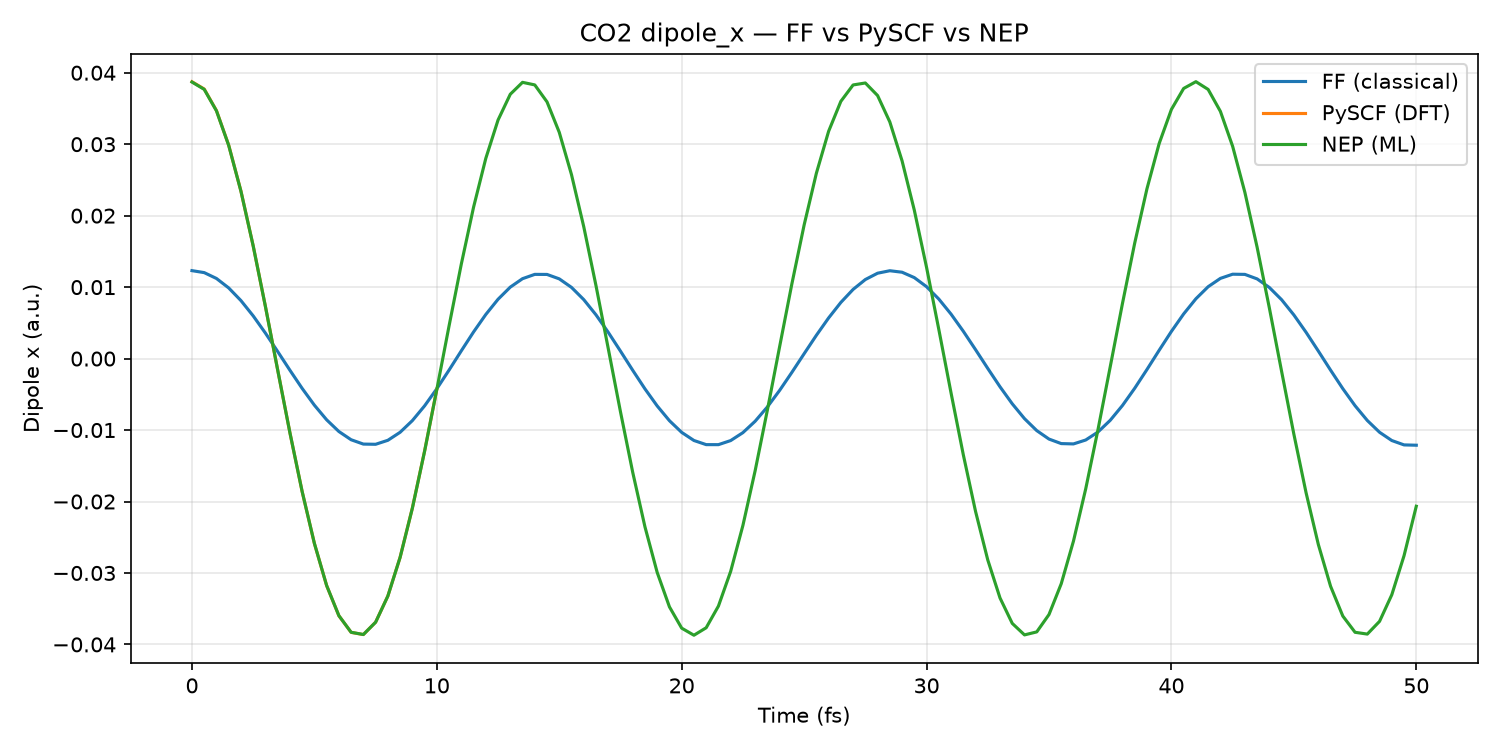
\includegraphics[width=0.80\linewidth]{dipole_comparison.png}
\caption{CO$_2$ dipole over time. FF gives smaller amplitude; PySCF and NEP
are nearly identical.}
\end{figure}

We then ran at coupling strengths $\lambda = 0, 0.1, 0.2, 0.3$ reproducing
Figure 1 of Bonini et al.\ 2024. At $\lambda = 0.1$ the asymmetric stretch
($\sim$2349 cm$^{-1}$) splits with $\Omega_R \approx 420$ cm$^{-1}$.

\begin{figure}[h]
\centering
\includegraphics[width=0.85\linewidth]{stacked_spectra.png}
\caption{Stacked IR spectra of CO$_2$ at four coupling strengths. The peak
splits into LP and UP as $\lambda$ increases. Matches Bonini et al.\ 2024.}
\end{figure}

\newpage

\section*{H$_2$O}

We ran water using PySCF only (no NEP model exists for H$_2$O). The cavity was
tuned to the bend mode at 1584 cm$^{-1}$, polarisation along $\hat{z}$.
2000 steps at 0.5 fs timestep, Hanning-windowed FFT.

\begin{figure}[h]
\centering
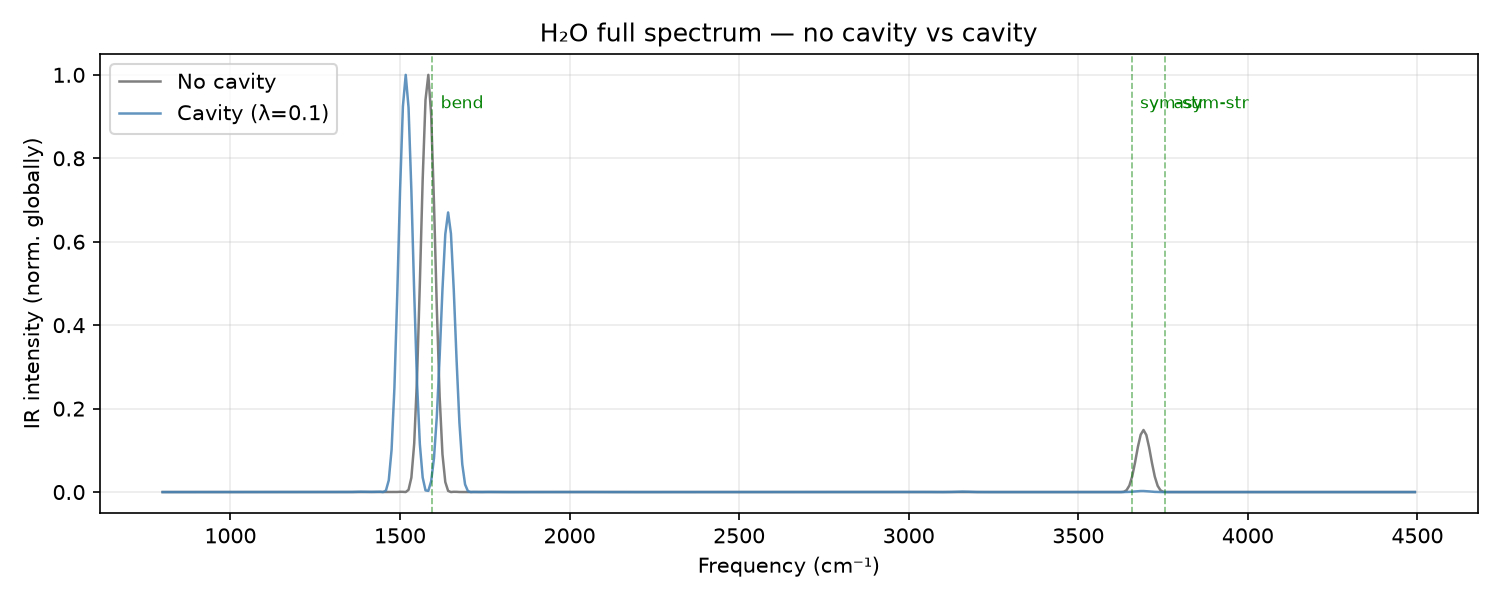
\includegraphics[width=0.90\linewidth]{h2o_full_hanning.png}
\caption{Full H$_2$O spectrum: no cavity (grey) vs cavity (blue). The bend
splits in the cavity run. The O--H stretch at 3657 cm$^{-1}$ is unaffected
--- cavity coupling is frequency-selective.}
\end{figure}

\begin{figure}[h]
\centering
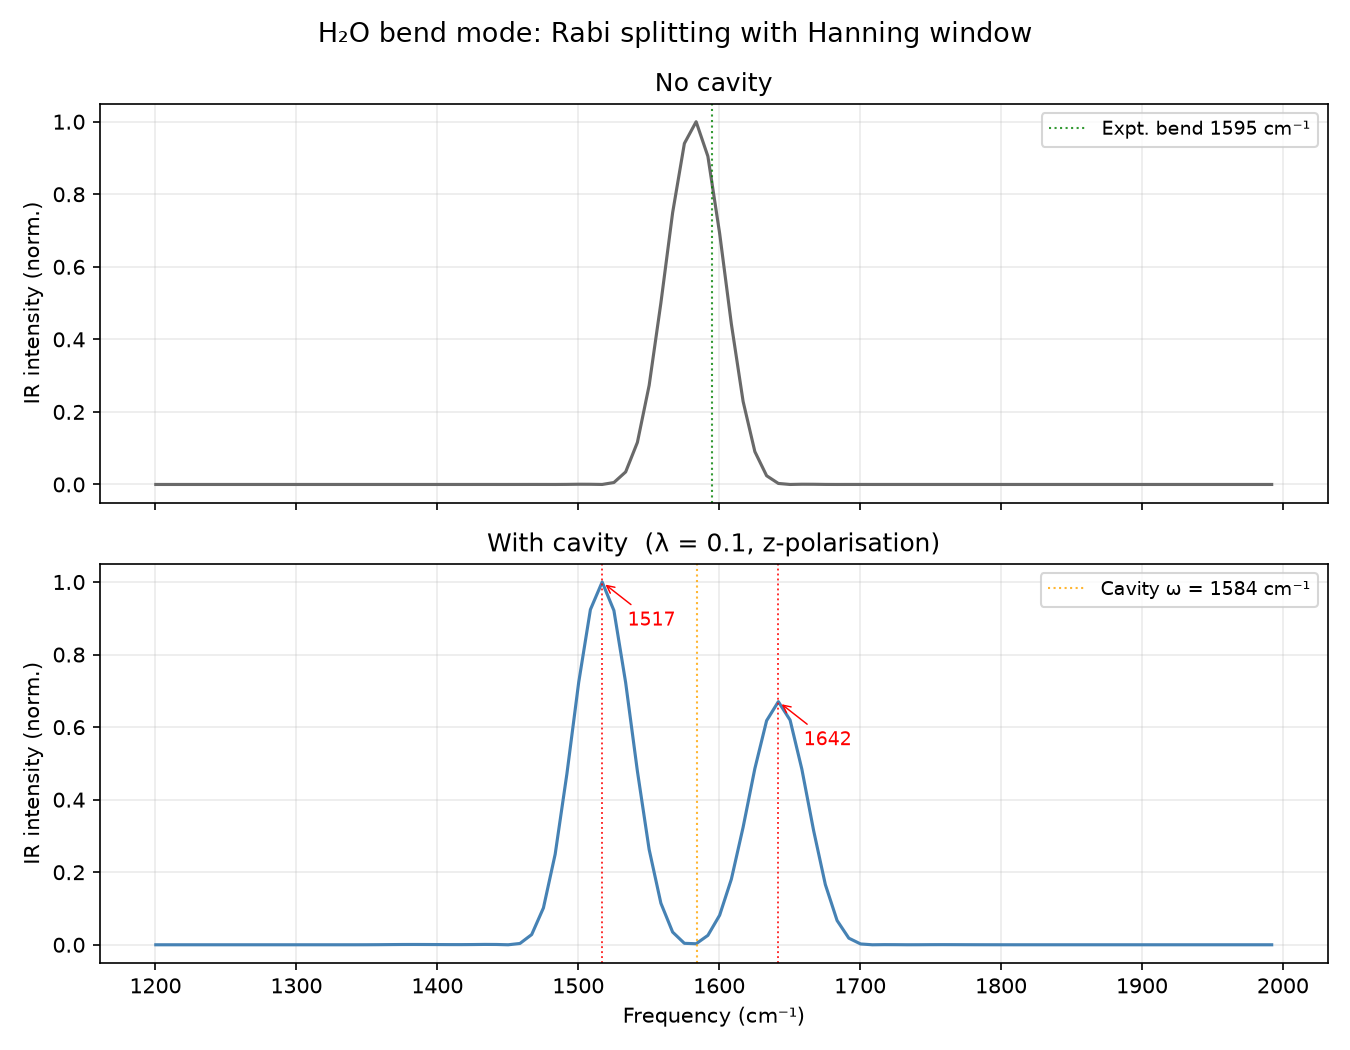
\includegraphics[width=0.90\linewidth]{h2o_bend_hanning.png}
\caption{Bend region in detail. Top: bare molecule, single peak at
$\sim$1580 cm$^{-1}$. Bottom: cavity run showing clear LP/UP splitting.}
\end{figure}

\begin{center}
\begin{tabular}{ll}
\hline
Lower polariton (LP) & 1517 cm$^{-1}$ \\
Upper polariton (UP) & 1642 cm$^{-1}$ \\
\textbf{Rabi splitting} & \textbf{125 cm$^{-1}$} \\
\hline
\end{tabular}
\end{center}

H$_2$O splits less than CO$_2$ (125 vs 420 cm$^{-1}$) because the water bend
has a smaller dipole derivative than the CO$_2$ asymmetric stretch.

\hrule
\vspace{1em}

\textbf{Next:} liquid water with LAMMPS --- 216 molecules, collective splitting
scales as $\sqrt{N}$, so $\sim$15$\times$ the single-molecule result.

\end{document}